\newcommand{\figGCcountermondelworldsfont}{\fontsize{8pt}{8pt}\selectfont}

\begin{tikzpicture}[scale=0.8]      
  
  % WORLDS  
  % w0
  \draw[fill] (0,-0.5) circle (3pt)
  +(0,-0)   node (w0)  {}  % used to label the circle 
  +(0,-0.3) node  {\figGCcountermondelworldsfont $w_0$}
  ;
  
  % w1 
  \draw[fill]  (-4,1) circle (3pt)
  +(0,0)   node (w1)  {}  % used to label the circle 
  +(-0.6,0)  node  {\figGCcountermondelworldsfont $w_1$} 
  +(0,0.4) node  {
    \begin{minipage}{10ex}\figGCcountermondelworldsfont
      \[
      \begin{array}{l}
        p=1/2\\[.2ex]
        q = 1/2-1/3\\[6ex]
      \end{array}
      \]
    \end{minipage}
  }
  ;
  
  % w2
  \draw[fill] (-1,1) circle (3pt)
  +(0,0)   node (w2)  {}  % used to label the circle 
  +(-0.6,0) node{\figGCcountermondelworldsfont $w_2$}
  +(0,0.4) node{
    \begin{minipage}{10ex}\figGCcountermondelworldsfont
      \[
      \begin{array}{l}
        p=1/2\\[.2ex]
        q= 1/2-1/4\\[6ex]
      \end{array}
      \]
    \end{minipage}
  }
  ;
  
  % w3
  \draw[fill] (2,1) circle (3pt)
  +(0,0)   node (w3)  {}  % used to label the circle 
  +(-0.6,0) node{\figGCcountermondelworldsfont $w_3$}
  +(0,0.4) node{
    \begin{minipage}{10ex}\figGCcountermondelworldsfont
      \[
      \begin{array}{l}
        p=1/2\\[.2ex]
        q= 1/2-1/5\\[6ex]
      \end{array}
      \]
    \end{minipage}
  }
  ;
  
  % DOTS
  
  \draw[fill] (3.5,1) node{.....}  ; 
  
 

 % EVALUATIONS

  \draw (4,-0.6) node{\begin{minipage}{27ex}\figGCcountermondelworldsfont
      $\Diam p= 1/2$
      \\[.5ex]
      $\Diam q = 1/2$ \tb{(non witnessed)}
      \\[.5ex]
      $\Diam(p \to  q) = 1/2$  \tb{(non witnessed)}
    \end{minipage}};

  \draw (0,-1.9) node (eval) {
    \begin{minipage}{25ex}\figGCcountermondelworldsfont
      \ggbox{$\overset{\tm{1}}{(\Diam p \to \Diam q)} \;\to\;
        \overset{\tm{0}}{\neg \Diam q} \,\lor\,\overset{\tm{1/2}}{\Diam(p\to q)}\,=\, 1/2$}
    \end{minipage}
  }; 
        

 % ARROWS
  \draw[magenta,->] (w0) -- (w1) node[midway,above, xshift=-1em,yshift=-2ex] {\figGCcountermondelworldsfont 1};
  \draw[magenta,->] (w0) -- (w2) node[midway, above,xshift=.2em] {\figGCcountermondelworldsfont  1}  ;
  \draw[magenta,->] (w0) -- (w3) node[midway, above, xshift=0.5em,yshift=-2ex] {\figGCcountermondelworldsfont 1} ;
  
 \draw[blue,thick,->] (w0.west)  .. controls +(-1.5,0) and +(-1.5,0) ..  (eval.west);
  

  
\end{tikzpicture}



%%% Local Variables: 
%%% mode: latex
%%% TeX-master: "slides_GoedelWitnessed_aiml2026"
%%% End: 
